%standard 13.2


%start_of_questions



%new_question
%%%%%%%%%%%%%%%%%%%%%
	% Problem 3
	% Difficulty: 2
%%%%%%%%%%%%%%%%%%%%%
	\item
		Write a class for a \textbf{LinearEquation} with the instance variables and methods listed 
		below.\\ A linear equation is of the form $y = mx + b$, where $m$ is the slope and $b$ is 
		the $y$-intercept.

		\begin{minipage}[t]{0.65\textwidth}
				For example:
			\begin{itemize}
				\item $y_1 = 2x + 3$
				\item $y_2 = -x + 5$
			\end{itemize}
			You should be able to add two equations together:
			\begin{itemize}
				\item $y_1 + y_2 = (2 - 1)x + (3 + 5) = x + 8$
			\end{itemize}
		\end{minipage}
		\hfill
		\begin{minipage}[t]{0.32\textwidth}
			\vspace{0.2em}
			\begin{flushright}
				\begin{tabular}{|l|}
					\hline
					LinearEquation \\ \hline
					m (slope) \\
					b (y-intercept) \\ \hline
					\_\_init\_\_ \\
					%evaluate(x) \\
					\_\_add\_\_ \\
					\_\_str\_\_ \\ \hline
				\end{tabular}
			\end{flushright}
		\end{minipage}
		
		Your class should support:
		\begin{itemize}
			\item Creating a linear equation with slope and y-intercept
			%\item Evaluating the equation at a given $x$ using the \texttt{evaluate(x)} method
			\item Adding two equations using the \_\_add\_\_ method
			\item Printing a readable version of the equation
		\end{itemize}
		
		Once you have created the class, add code that:
		\begin{itemize}
			\item Instantiate two linear equations
			%\item Evaluates one at a specific $x$ value
			\item Add them together
			%\item Handles invalid inputs (e.g., non-numeric $x$ in evaluate)
			\item print a readable version of one of the LinearEquations you created.
		\end{itemize}



%new_question
%%%%%%%%%%%%%%%%%%%%%
	% Problem 4
	% Difficulty: 2
%%%%%%%%%%%%%%%%%%%%%
	\item
		Write a class for a \textbf{Time} object with the instance variables and methods listed 
		below.\\
		Time can be represented in hours and minutes (e.g., 2 hours and 45 minutes). \\
		When adding times, make sure minutes are correctly carried into hours.

		\begin{minipage}[t]{0.65\textwidth}
			For example:
			\begin{itemize}
				\item $t_1 = 1$ hour $30$ minutes
				\item $t_2 = 2$ hours $45$ minutes
				\item $t_1 + t_2 = 4$ hours $15$ minutes 
					(because $30 + 45 = 75$ minutes, which becomes $1$ hour $15$ minutes)
			\end{itemize}

		\end{minipage}
		\hfill
		\begin{minipage}[t]{0.32\textwidth}
			\vspace{.2em}
			\begin{flushright}
				\begin{tabular}{|l|}
					\hline
					Time \\ \hline
					hours \\
					minutes \\ \hline
					\_\_init\_\_ \\
					\_\_add\_\_ \\
					\_\_str\_\_ \\ \hline
					%to\_minutes \\ 
				\end{tabular}
			\end{flushright}
		\end{minipage}
		
		Your class should support:
		\begin{itemize}
			\item Creating a time object with hours and minutes
			\item Adding two times using the \_\_add\_\_ method 
				%(properly handling minutes overflow)
			\item Printing time in a readable format (e.g., \csq{2h 45m})\\
				Hint: you don't need to consider days. You can have 30 hours.
			%\item Converting total time to just minutes using \texttt{to\_minutes()}
		\end{itemize}

		Once you have created the class, add code that:
		\begin{itemize}
			\item Creates two time objects
			\item Adds them together
			\item Prints the result
			%\item Shows the total number of minutes
			%\item Includes error handling for negative values or invalid types
		\end{itemize}



%new_question
%%%%%%%%%%%%%%%%%%%%%
	% Problem 5
	% Difficulty: 2
%%%%%%%%%%%%%%%%%%%%%
	\item
		Write a class for an \textbf{RGBColor} with the instance variables and methods listed 
		below. Colors on a screen are often represented using Red, Green, and Blue components 
		(values from 0 to 255).\\
		Colors can be added together by taking the average of adding each component.

		\begin{minipage}[t]{0.7\textwidth}
			Some examples of RGB colors:
			\begin{itemize}
				\item $c_1 = (170,\ 150,\ 200)$
				\item $c_2 = (30,\ 100,\ 60)$
				\item $c_3 = c_1 + c_2 = (\frac{170+30}{2},\ \frac{150+100}{2},\ \frac{200+60}{2})$ 
					becomes $(100,\ 125,\ 130)$
			\end{itemize}
		
			Your class should support:
			\begin{itemize}
				\item Creating a color with red, green, and blue values (each from 0 to 255)
				\item Adding two colors using the \_\_add\_\_ method (cap each result at 255)
				\item Printing the color in a readable format (e.g.,\csq{RGB(150, 200, 255)})
			\end{itemize}
		\end{minipage}
		\hfill
		\begin{minipage}[t]{0.25\textwidth}
			\vspace{.2em}
			\begin{flushright}
				\begin{tabular}{|l|}
					\hline
					RGBColor \\ \hline
					r (red) \\
					g (green) \\
					b (blue) \\ \hline
					\_\_init\_\_ \\
					\_\_add\_\_ \\
					\_\_str\_\_ \\ \hline
				\end{tabular}
			\end{flushright}
		\end{minipage}
		
		After writing the class, create three colors and write code to add them together.
		Print the result.

	

%new_question
%%%%%%%%%%%%%%%%%%%%%
	% Problem 6
	% Difficulty: 2
%%%%%%%%%%%%%%%%%%%%%
	\item
		Write a class for a \textbf{RationalNumber} with the instance variables and methods 
		listed below.\\
		A RationalNumber is a number that can be expressed as the ratio of two integers: 
		$\dfrac{a}{b}$, where $b \ne 0$.

		\begin{minipage}[t]{0.65\textwidth}
			Some examples of RationalNumber addition include:
			\begin{itemize}
				\item $\dfrac{1}{3} + \dfrac{1}{2} = \dfrac{5}{6}$ (not $0.8333\ldots$)
				\item $\dfrac{2}{5} + \dfrac{1}{5} = \dfrac{3}{5}$
			\end{itemize}
		\end{minipage}
		\hfill
		\begin{minipage}[t]{0.32\textwidth}
			\vspace{.2em}
			\begin{flushright}
				\begin{tabular}{|l|}
				\hline
				RationalNumber \\ \hline
				numerator \\
				denominator \\ \hline
				\_\_init\_\_ \\
				\_\_add\_\_ \\
				\_\_str\_\_ \\ \hline
				\end{tabular}
			\end{flushright}
		\end{minipage}
		
		Your class should support:
		\begin{itemize}
			\item Creating a rational number with a numerator and denominator
			\item Adding two rational numbers using the \_\_add\_\_ method 
			\item Printing a readable version (e.g., as a fraction)
		\end{itemize}
		
		Hint: To add fractions, find a common denominator.\\
		For example, $\dfrac{1}{3} + \dfrac{1}{2} = \dfrac{2}{6} + \dfrac{3}{6} = \dfrac{5}{6}$.\\
		\newline
		After writing the class, create two rational numbers and demonstrate adding and printing.




%new_question
%%%%%%%%%%%%%%%%%%%%%
	% Problem 10
	% Difficulty: 2
%%%%%%%%%%%%%%%%%%%%%
	\item
		Write a class for a \textbf{Rectangle} with the instance variables and methods 
		listed below.\\
		A Rectangle has a width and a height. You should be able to calculate its area	and multiply 
		a Rectangle by an integer. The result of multiplying by an integer should be that the height 
		and width of the current Rectangle are multiplied (modified) by the integer value.
		%When a rectangle is multiplied by an integer the result should be that the current 
		%rectangle has both its height and width modified by that integer value. 

		\begin{minipage}[t]{0.7\textwidth}
			Some examples:
			\begin{itemize}
				\item $r_1 = \text{width: } 4,\ \text{height: } 5$
				\item $r_2 = \text{width: } 3,\ \text{height: } 2$
				\item $r_1 * 3 = \text{width: } 12,\ \text{height: } 15$
			\end{itemize}

			\begin{minipage}{0.25\textwidth}
				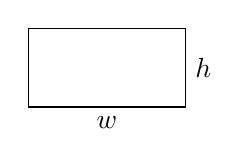
\begin{tikzpicture}
					\draw (0,0)  -| (2,1) 
						node[pos=0.25,below] {$w$} 
						node[pos=0.75,right] {$h$}
						-| (0,0);
				\end{tikzpicture}
			\end{minipage}
			{\Large $\longrightarrow$} \hspace*{2em}
			\begin{minipage}{0.65\textwidth}
				\begin{tikzpicture}
					\draw (0,0)  -| (6,3) 
						node[pos=0.25,below] {$3 \cdot w$} 
						node[pos=0.75,right] {$3 \cdot h$}
						-| (0,0);
				\end{tikzpicture}
			\end{minipage}
		\end{minipage}
		\hfill
		\begin{minipage}[t]{0.2\textwidth}
			\vspace{.2em}
			\begin{flushright}
				\begin{tabular}{|l|}
					\hline
					Rectangle \\ \hline
					width \\
					height \\ \hline
					\_\_init\_\_ \\
					area() \\
					%perimeter() \\
					\_\_mul\_\_ \\
					\_\_str\_\_ \\ \hline
				\end{tabular}
			\end{flushright}
		\end{minipage}
		
		Your class should support:
		\begin{itemize}
			\item Creating a rectangle with width and height.
			\item Calculating the area using \texttt{area()}.
				%and perimeter using \texttt{perimeter()}
			\item Multipying a rectangle by an integer using the  \_\_mul\_\_ method.
			\item Printing the rectangle in a readable format (e.g., \csq{Rectangle(4 x 5)})
		\end{itemize}
		
		Once you have created the class, add code that:
		\begin{itemize}
			\item Creates a rectangle
			\item Multiplies it by an integer.
			\item Prints the result
		\end{itemize}

%end_of_questions
%make sure to leave at least one blank line below

